\documentclass[]{article}

\usepackage[a4paper]{geometry}

\usepackage{lmodern}
\usepackage{amssymb,amsmath}
\usepackage{fixltx2e} % provides \textsubscript

\usepackage[T1]{fontenc}
\usepackage[utf8]{inputenc}

% straight quotes in verbatim environments
\usepackage{upquote}

\usepackage[defaultlines=4,all]{nowidow}

\usepackage{microtype}
\UseMicrotypeSet[protrusion]{basicmath} % disable protrusion for tt fonts

\PassOptionsToPackage{hyphens}{url} % url is loaded by hyperref

\usepackage[unicode=true]{hyperref}

% \hypersetup{
%             pdfborder={0 0 0},
%             breaklinks=true}

\usepackage{enumitem}
\setitemize{itemsep=0pt}
\setenumerate{itemsep=0pt}

% \urlstyle{same}  % don't use monospace font for urls

\usepackage{longtable,booktabs,multirow}

% Fix footnotes in tables (requires footnote package)
\IfFileExists{footnote.sty}{\usepackage{footnote}\makesavenoteenv{long table}}{}

\usepackage{graphicx,grffile}
\makeatletter
\def\maxwidth{\ifdim\Gin@nat@width>\linewidth\linewidth\else\Gin@nat@width\fi}
\def\maxheight{\ifdim\Gin@nat@height>\textheight\textheight\else\Gin@nat@height\fi}
\makeatother
% Scale images if necessary, so that they will not overflow the page
% margins by default, and it is still possible to overwrite the defaults
% using explicit options in \includegraphics[width, height, ...]{}
\setkeys{Gin}{width=\maxwidth,height=\maxheight,keepaspectratio}

% \setlength{\emergencystretch}{3em}  % prevent overfull lines

% Redefines (sub)paragraphs to behave more like sections
\ifx\paragraph\undefined\else
\let\oldparagraph\paragraph
\renewcommand{\paragraph}[1]{\oldparagraph{#1}\mbox{}}
\fi
\ifx\subparagraph\undefined\else
\let\oldsubparagraph\subparagraph
\renewcommand{\subparagraph}[1]{\oldsubparagraph{#1}\mbox{}}
\fi

\makeatletter
\let\_\relax
\DeclareRobustCommand{\_}{%
  \leavevmode\vbox{%
    \hrule\@width.5em
          \@height-.26ex
          \@depth\dimexpr.26ex+.28pt\relax}}
\makeatother

% set default figure placement to htbp
\makeatletter
\def\fps@figure{htbp}
\makeatother

\title{
  zeppelinOS:
  An open-source, distributed platform of tools and services on top of the EVM,
  to develop and manage smart contract applications securely \bigskip
}

\author{
  Manuel Araoz, Demian Brener, Teemu Paivinen, Alberto Gozzi \smallskip\\
  \normalsize \url{https://zeppelinos.org} \medskip
}

\date{August 2017}

\begin{document}

\maketitle

\begin{center}WORKING DRAFT\end{center}

  \bigskip

\begin{abstract}

The blockchain ecosystem has seen an explosion in new protocols
recently. These protocols promise to provide everything from traditional
transfer of value to decentralised file storage. This is an exciting
time as the blockchain industry can redesign and rebuild much of the
traditional internet infrastructure. We have an opportunity to make it
faster, easier and safer to deploy complex applications online, in a
decentralised environment.

However, the industry has been plagued by security breaches and it is
becoming clear that while the promise of blockchain technology is
phenomenal, we need to approach this technology with caution. At the
same time we want to make this technology as accessible as possible,
fueling innovation and accelerating the move to a decentralised, open
economy.

As an answer to these problems and opportunities, we propose
zeppelinOS, an operating system for decentralised applications.
zeppelinOS allows developers to easily build secure applications
that use and combine existing protocols. zeppelinOS is made up of five
distinct components: the kernel, the protocol marketplace, state
channels, the scheduler and off-chain tools. We also propose a new token
ZEP to fuel the zeppelinOS ecosystem. The token allows users to
operate any zeppelinOS application, is used as the primary governance
mechanism for upgrades and creates liquidity across protocols available
to developers in the marketplace.

\end{abstract}

\newpage

\tableofcontents

\newpage

\section{Introduction}

Decentralised applications often facilitate some kind of financial
exchange for services. Ensuring the security of this financial exchange
and the funds held in interacting applications/smart contracts is
imperative to the success of the blockchain ecosystem. Currently there
is little standardisation and no easy way to develop highly secure
applications easily. zeppelinOS is an open-source, distributed
platform of tools and services on top of a virtual machine, initially
EVM~\cite{evm}, to develop and manage smart contract applications securely.

\section{Elementary Components}

zeppelinOS is made up of five distinct components: the kernel, the
scheduler, the protocol marketplace, state channels and off-chain
tools.

\subsection{Kernel}

The Kernel is to act as the foundation layer of zeppelinOS, providing
an on-chain set of basic functionality and services for the smart
contracts that use the operating system, and supporting a distributed
upgrading mechanism powered by decentralized voting of ZEP token
holders. The upgradeability mechanism of the zeppelinOS Kernel will be
based on the proxy library pattern~\cite{proxylibs} and is described in
the Governance section.

The goal for the zeppelinOS Kernel is to provide a set of functions for
the smart contracts that run on top of it, requesting services from the
OS rather than re-implementing them from scratch. These functions will
be available as an on-chain standard library of reusable contracts and
functions, heavily inspired by OpenZeppelin~\cite{openzeppelin}, and held to the
same security standards.

Examples of things developers will be able to do with these libraries
include:

\begin{itemize}
\item
  {Create and customize a ERC20 Token.}
\item
  {Create a capped, refundable, and/or whitelisted crowdsale contract.}
\item
  {Create a trustless bug bounty.}
\item
  {Create pausable, ownable, and balance-limited contracts.}
\item
  {Set up a token vesting or token locking contract.}
\end{itemize}

\begin{figure}
  \centering
  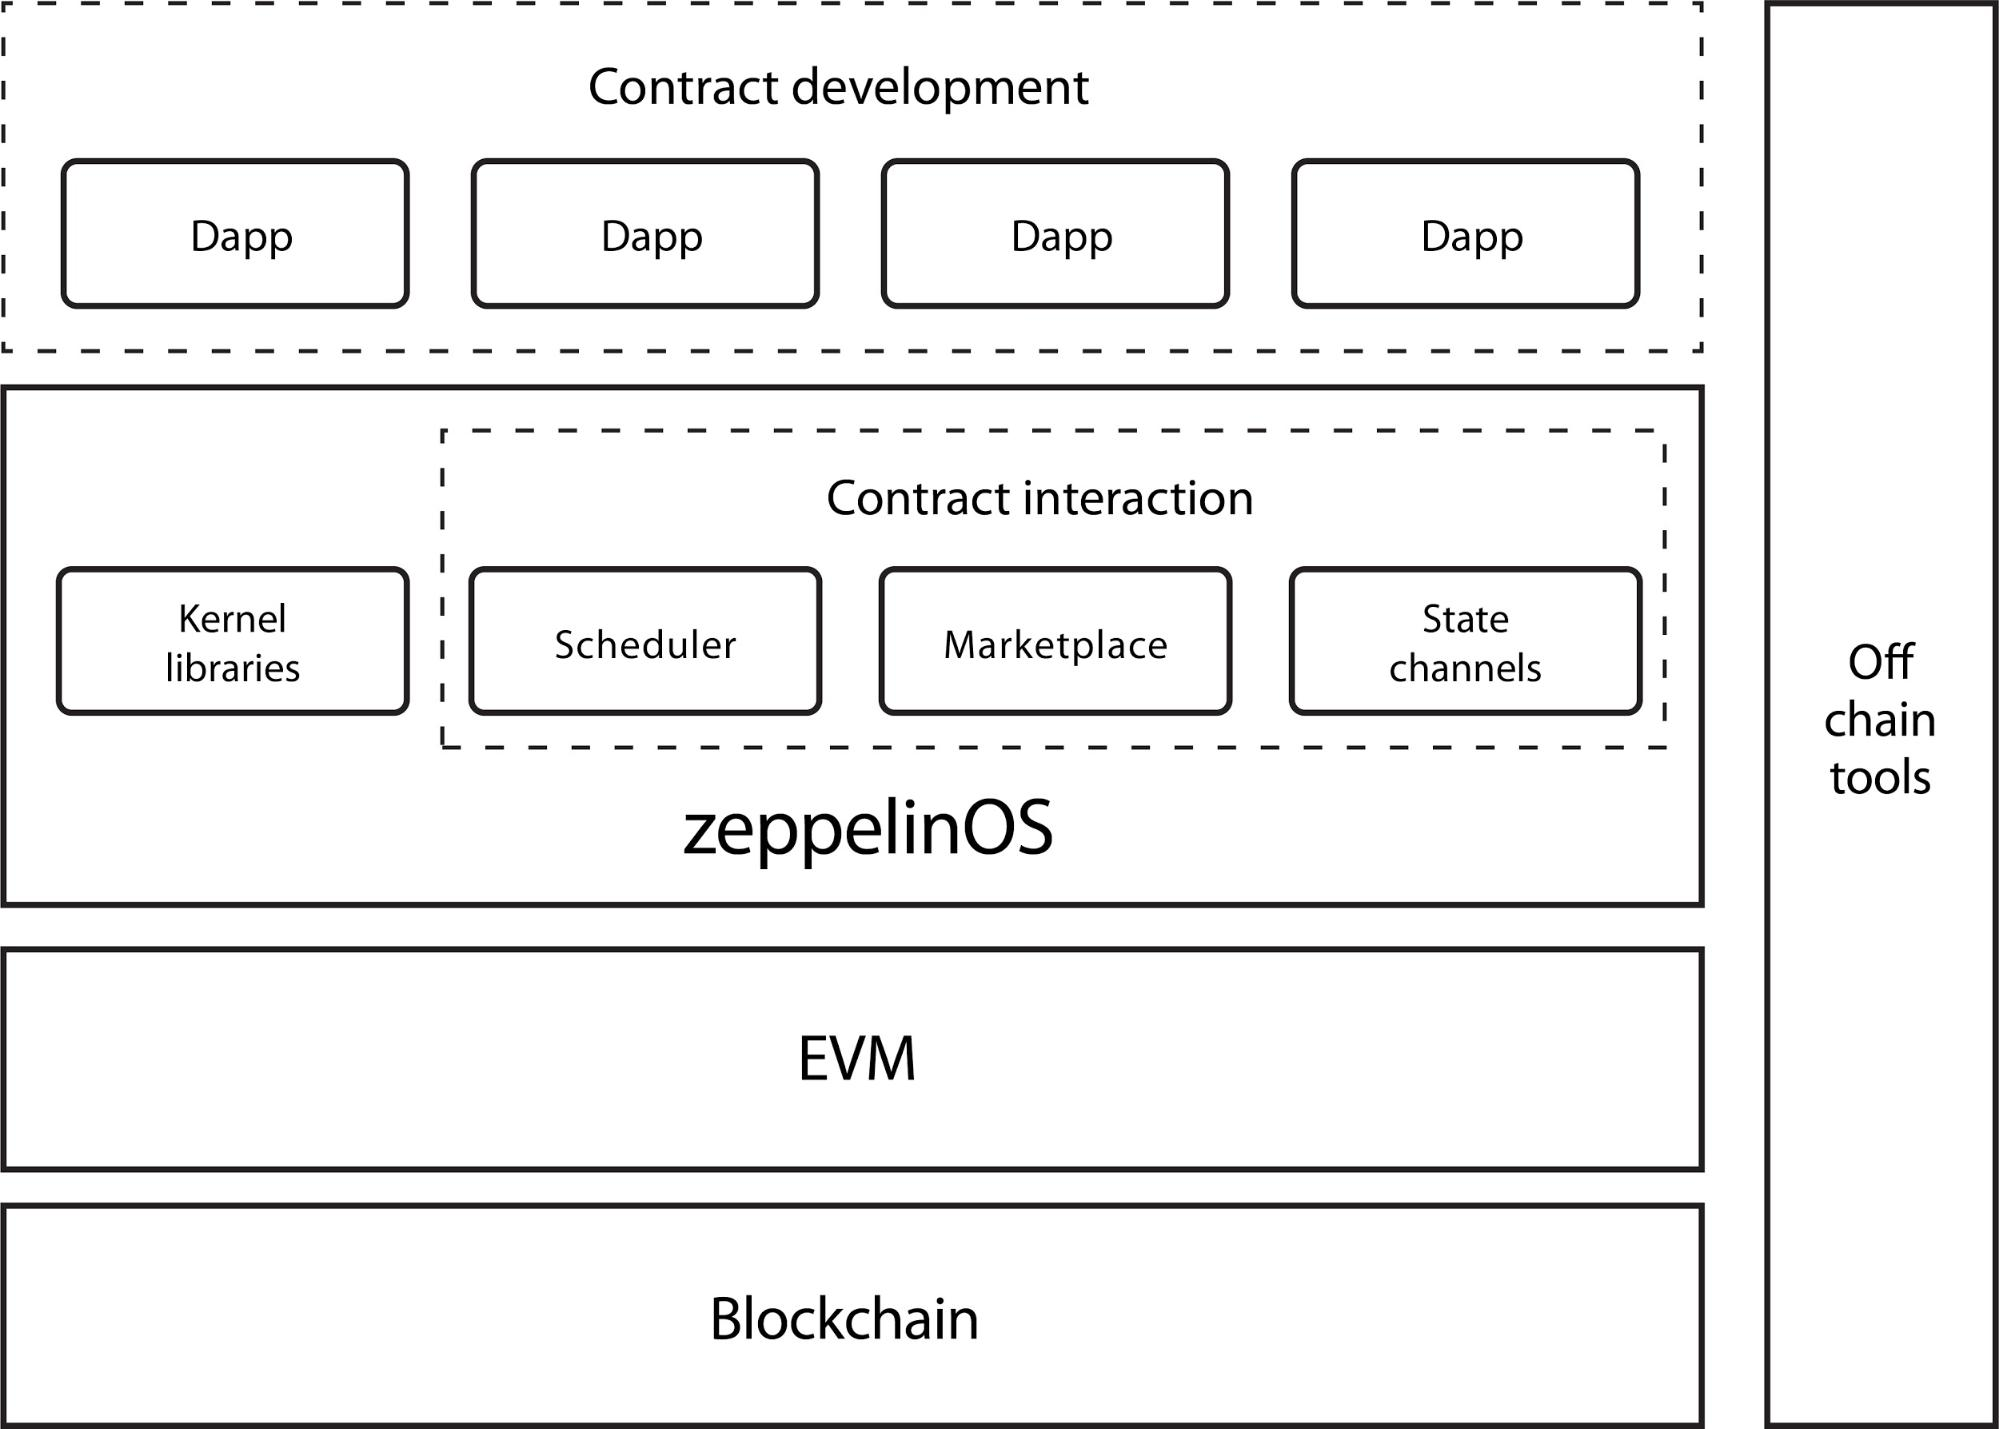
\includegraphics[width=0.75\linewidth]{images/image6.jpg}

  \caption{zeppelinOS in the broader blockchain stack.}
\end{figure}

\subsubsection{Standard Library}

zeppelinOS will provide an on-chain standard library of reusable
contracts and functions. The goal for the zeppelinOS Kernel is to
provide a set of functions to act as system calls for the smart
contracts that run on top of it, thus requesting services from the OS
rather than reimplementing them.

\subsubsection{Security Patches}

Being a layer that smart contracts communicate with on-chain, we open
up the possibility of delivering upgrades to zeppelinOS users. This
enables rolling out security mitigations and patches as soon as a
vulnerability is found, instantly protecting all users of zeppelinOS.

To make upgrading happen in a decentralized manner, users will
participate in a shared vouching system powered by ZEP tokens, and
will be incentivized to review patches and vouch for their
correctness. Such a mechanism is necessary to avoid the possibility of
a centralized party upgrading (i.e. changing) all contracts using the
optional automatic upgrade system in the OS without any control from
the community, while providing a mechanism of fast response in the event
of a critical security issue if it is acknowledged by the majority.

\subsubsection{Continuous Improvement}

Through the same upgradeability mechanism, zeppelinOS will be able
to remain in a state of continuous development. This includes the
improvement of existing zeppelinOS components, as well as the
development of new ones that are identified as necessary by the
community. This allows both the service layer and the contracts that
make use of it to always include state-of-the-art smart contract code.

\subsubsection{Attack Response}

Experience has shown that bugs will always be found in a codebase. As smart
contracts become more complex, the probability of bugs becomes
larger~\cite{schneier}, and with it comes a greater possibility of being the
target of an attack.

To be prepared for it, we will provide a toolbox for attack response.
Triggering an emergency pause, reverting to a previous uncompromised
state, or forking a contract are some of the possibilities.

\subsubsection{Contract Upgradeability}

In addition to having upgradeability of the zeppelinOS Kernel itself,
the underlying implementation will be made available to users of the OS
to enable upgradeability of their own smart contracts. This allows
rolling out contract-specific security patches, as well as the
progressive deployment of features.

\subsection{Scheduler}

Contract code execution is synchronous and linear, having the
possibility to call other contracts but restrained to a single and
contiguous execution thread. To support more complex operations,
applications require off-chain infrastructure, defeating the very
purpose of fully decentralized applications.

As a means to support richer execution models, the OS shall provide,
through the usage of a standardised set of signaling events, a
bounty-based smart contract async execution scheduler, where different
parties can offer to execute async operations and securely call back
into the contract to resume operations. This also opens the way to
standard mechanisms for requesting data from trusted authoritative
sources, by adding a validation on the callback originator to ensure the
response is provided by a secure oracle.

In order to accomplish this, the OS will define the required standards
and provide code for simplifying their adoption, for both the scheduler
clients and the providers who wish to offer the execution of async
operations, effectively setting up nodes that power the distributed
scheduling network.

\subsection{State Channels}

Though distributed and secure, in-chain transactions are limited in
frequency and cost by block mining times and fees. This caused the
emergence of alternate off-chain transaction systems that could be
consolidated back to the blockchain after multiple operations, with
State Channels~\cite{statechan} being one of the latest proposals for
intercommunication between two or more peers, verified and consolidated
by a smart contract acting as a judge.

The OS shall incorporate state channel support through common protocol
specs and reference implementations, plus all the on-chain
infrastructure necessary for discovery, arbitration and consolidation of
state channels. Besides providing a cheaper communication mechanism,
this also leaves the door open for future direct integration with
off-chain state payment networks in the platform.

\subsection{Protocol Marketplace}

Much as traditional mobile app marketplaces act as central hubs for
mobile users to browse and purchase available services, one of the
central features of zeppelinOS is a marketplace for contracts, where
services can be purchased and integrated into other applications.

Though smart contracts are currently quite limited in their
interactions with the off-chain world, the advent of services that
provide the bridge to execute side-chain effects can offer true
decentralized applications the power to run entirely on zeppelinOS.
Examples of such services are file storage, mail sending, push
notifications, off-chain intensive computation, machine-learning
services, etc.

The interaction with such services shall be facilitated through
different standard execution models powered by the OS, and payments
executed with the platform ZEP tokens, thus enabling an effective
in-OS economy between service providers and their client applications.
This model also improves security as interactions with various protocols
is standardized and public allowing for auditing on a continuous basis.

\subsubsection{Protocol Proxies}

Applications built on zeppelinOS may include one or more external
protocols via the marketplace. As the native token ZEP is used to
operate applications built on the platform, there needs to be a
mechanism by which the proxy for an external protocol converts ZEP into
whichever token is required to use the external protocol. The
marketplace thus needs to have some kind of exchange mechanism. We
propose two complementary methods for achieving this, both of which
are explored below. 

\paragraph{Exchange}

This method is relatively simple in that it does not require the
developer of a marketplace integration to apply funds to ensuring the
functioning of their application. The exchange method would utilise
existing exchange infrastructure to manage conversions between ZEP and
other tokens, allowing for real-time conversions within the
application smart contracts.

Each protocol integration would connect to a zeppelinOS exchange integration
allowing for the efficient conversion of ZEP into other protocol tokens. In the
future, competitive mechanics can be added to the exchange process by creating
a mechanism for exchanges to compete for any given transaction. If opened up to
the market, traders could provide this service and benefit from the spread
attainable by performing market making operations.

\paragraph{Buffer}

The other option for providing marketplace exchange, this time without
using an actual exchange, requires the developer of the integration to
load tokens of the external protocol to a smart contract, creating a
buffer. These tokens will be used to pay for protocol services as users
pay for services in the application using ZEP. The smart contract will
have an oracle which dictates the exchange rate for converting ZEP to
the external token. The developer then receives ZEP and spends the
external tokens. The developer of the integration thus functions like a
market maker. 

This method may require the developer of an integration to hold
significant amounts of the protocol token, which is not ideal for
keeping barriers to entry low. However, this method could also allow the
developer of the integration to charge a spread on the exchange to
generate revenue. Eventually such a spread would decrease to the lowest
point where it makes sense to provide such a service. On the user side,
this competitive tendency to lower cost, will lead to the best
achievable prices over time.

\begin{figure}
  \centering
  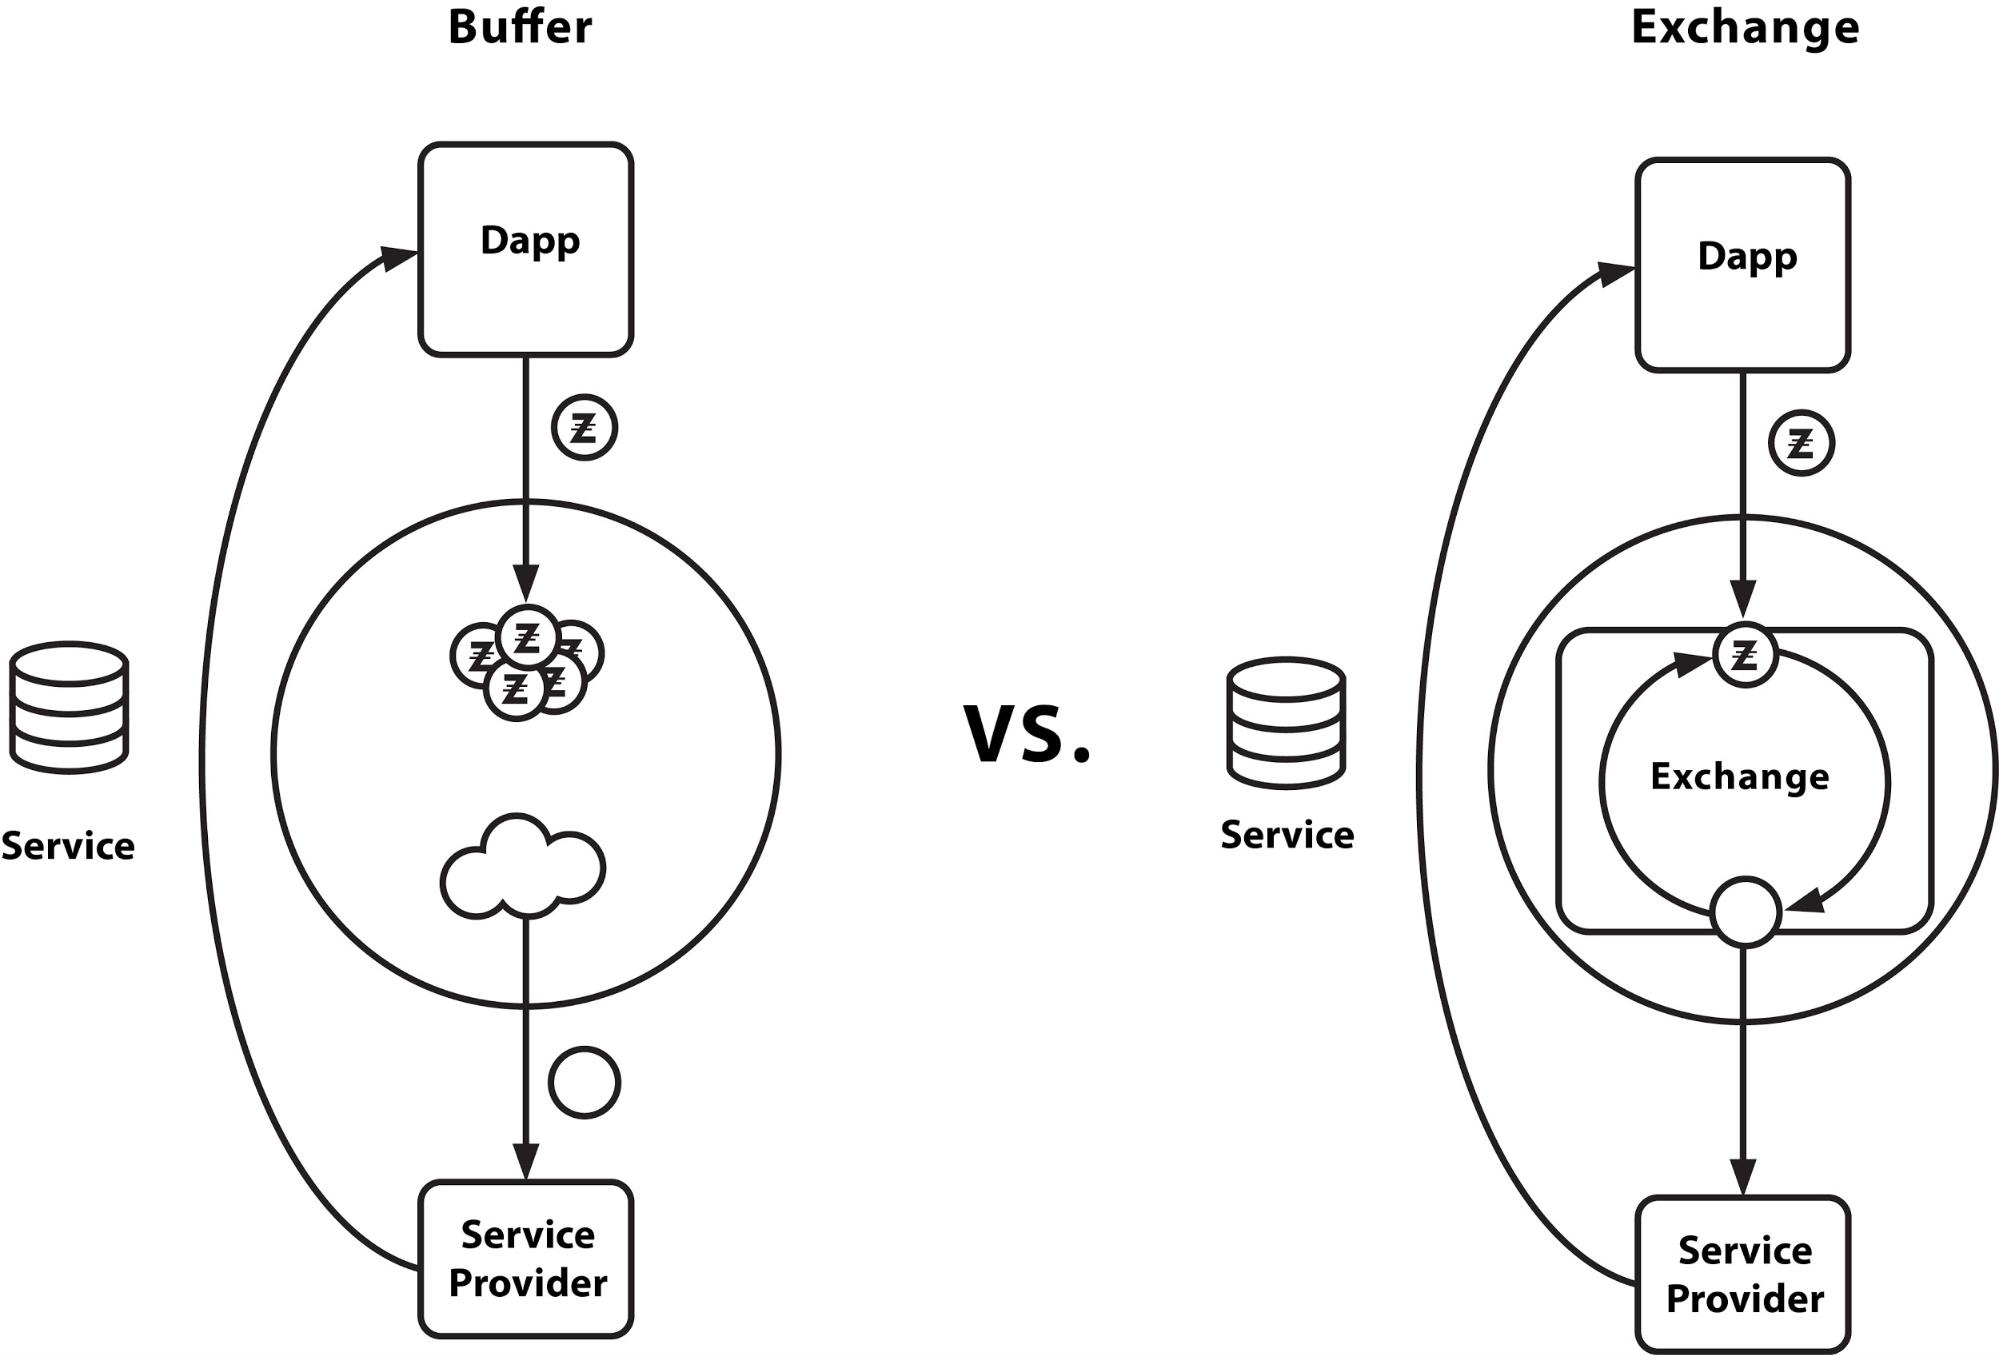
\includegraphics[width=0.65\linewidth]{images/image3.jpg}
  \caption{The alternative mechanisms for payments to external protocols.}
\end{figure}

\paragraph{Considerations and Pending Challenges}

\begin{itemize}

  \item
    The buffer method requires the holding of protocol tokens in a smart
    contract. Some protocols may not support smart contracts, thus making it
    difficult to use the buffer method for these protocols in creating proxies
    for the marketplace. To solve this problem, we will build bridges to allow
    users of the OS to interact with other blockchain platforms (e.g. Tezos).

  \item
    The buffer method requires the developer of the marketplace integration to
    hold some amount of the respective protocol's tokens, possibly increasing
    barriers to entry.

\end{itemize}

\subsubsection{Marketplace Review}

All submissions to the marketplace will be carefully reviewed to ensure
the highest quality and security. Initially this review process will be
conducted by the Zeppelin Solutions~\cite{zeppelinsols} team, along with a public
review with a bug bounty. A centralised marketplace review has
benefits in terms of maintaining quality of contents and efficiency of
the review process, but history tells us it also allows the controlling
party to exert non-competitive influence~\cite{apple}. We understand this
problem and are fully committed to transitioning into a decentralised
review model once the most suitable model is found.

\paragraph{Considerations and Pending Challenges}

\begin{itemize}

  \item
    Decentralising marketplace review needs to be efficient, scalable and
    maintain a high quality of accepted submissions. This can potentially
    be achieved using a delegated proof-of-stake model, where the
    delegates are incentivised to review submissions and act along
    guidelines voted on by the community.

\end{itemize}

\subsection{Off-Chain Tools}

As an addition to the on-chain services offered by zeppelinOS, the
platform will provide a set of off-chain tools aimed at simplifying the
development, debugging, testing, deployment, and monitoring of
decentralized applications.

\subsubsection{Analytics \& Monitoring}

Contract transactions and events provide invaluable insight on the
usage of a deployed application, analogous to end-user actions and
events performed on a web page. As such, an off-chain analytics
dashboard can aggregate on-chain generated contracts events for research
on their usage. Also, by tracking from which node each transaction is
originated, it's possible to obtain information on how end-users actually
connect to the network to interact with the contracts.

The other side of tracking contract-generated events and transactions
is monitoring the health of each contract, by keeping record of the
transaction error rate and failure-associated events, thus triggering
alerts through both general and per-contract defined rules.

\subsubsection{Heroku~\cite{heroku} for Decentralized applications}

In order to simplify the deployment process, the platform will provide
the necessary development tools to facilitate the transition from
writing smart contracts high-level code to running in-chain distributed
applications. Submitting the code to the platform shall trigger a
testing and analysis process, described in the following sections, which
will be followed by an actual deployment to the blockchain, or an
upgrade powered by the aforementioned mechanisms, thus minimizing the
devops complexity of dapps for programmers.

The Platform as a Service approach also includes acting as a one-stop
platform for integration with other contracts, providing a user
interface for the discovery and management of marketplace-offered
services, so dapp owners can plug-and-play different infrastructure
building blocks. Like IFTTT~\cite{ifttt} recipes for smart contracts.

\subsubsection{Continuous Integration for Contracts}

Automated testing through continuous integration providers has become an
industry standard, as a means to increase the confidence on the project health
by checking its tests in a separate environment at every stage of development.
However, this requires a testing environment with conditions as similar as
possible as the production one. As such, zeppelinOS shall provide the required
services for effectively testing smart contracts and their interactions with
other services in a continuous integration fashion, including replayability of
previous transactions using the updated codebase to compare generated outcomes.

\subsubsection{Automated Code Analysis}

Static analysis is a long-running research field in academia, with
occasional ports to industry-level tools, despite its enormous benefits
towards the assurance of correctness and its ability to identify
potential bugs. Given the high security requirements of decentralized
applications, applying these strategies to smart contracts code is a
must, and an area to be continuously researched and improved.

Having access to the code powering the smart contracts applications,
zeppelinOS shall offer automated code analysis services with
increasingly powerful rules and techniques, preventing inadvertently
deploying potentially unsecure code, and alerting owners of existing
running contracts of newly found vulnerabilities.

\subsubsection{Meta-chain Information Provider}

zeppelinOS shall provide a standard way to access, from a smart
contract, information on the blockchain currently unavailable from
on-chain apps, such as current ETH price, gas price, transaction pool
size, average mining block times, etc.

This could be implemented either as an oracle providing information to
requests signalled as events, as described in the scheduler, or as calls
to Kernel contracts which are continuously updated by a trusted external
source with the latest chain stats.

\subsubsection{Inter Contract Communication}

The OS shall provide various mechanisms for inter-contract
communication and networking, such as publish-subscribe messaging,
message queues, and shared storage.

\section{ZEP Token}

Crypto-economic protocols create financial incentives to drive a
network of rational actors to co-ordinate their behaviour towards a
common goal. Often the alignment of incentives is achieved by
introducing a native token. In the case of zeppelinOS the native token
is ZEP and its goal is two-fold: (1) to ensure secure
deployment of upgrades to the zeppelinOS technology platform and (2)
financially incentivise the creation of liquidity against token
protocols in the marketplace. On a more general level, the goal is to
align network incentives to establish, grow and maintain an ecosystem
for easy development of secure decentralised applications. As a side
effect of these incentives, ZEP will be the standard token for all
applications built using zeppelinOS. With ZEP we move the exchange
functionality down the stack to a standardized solution, removing
friction from both the consumer and the
developer.

\begin{figure}
  \centering
  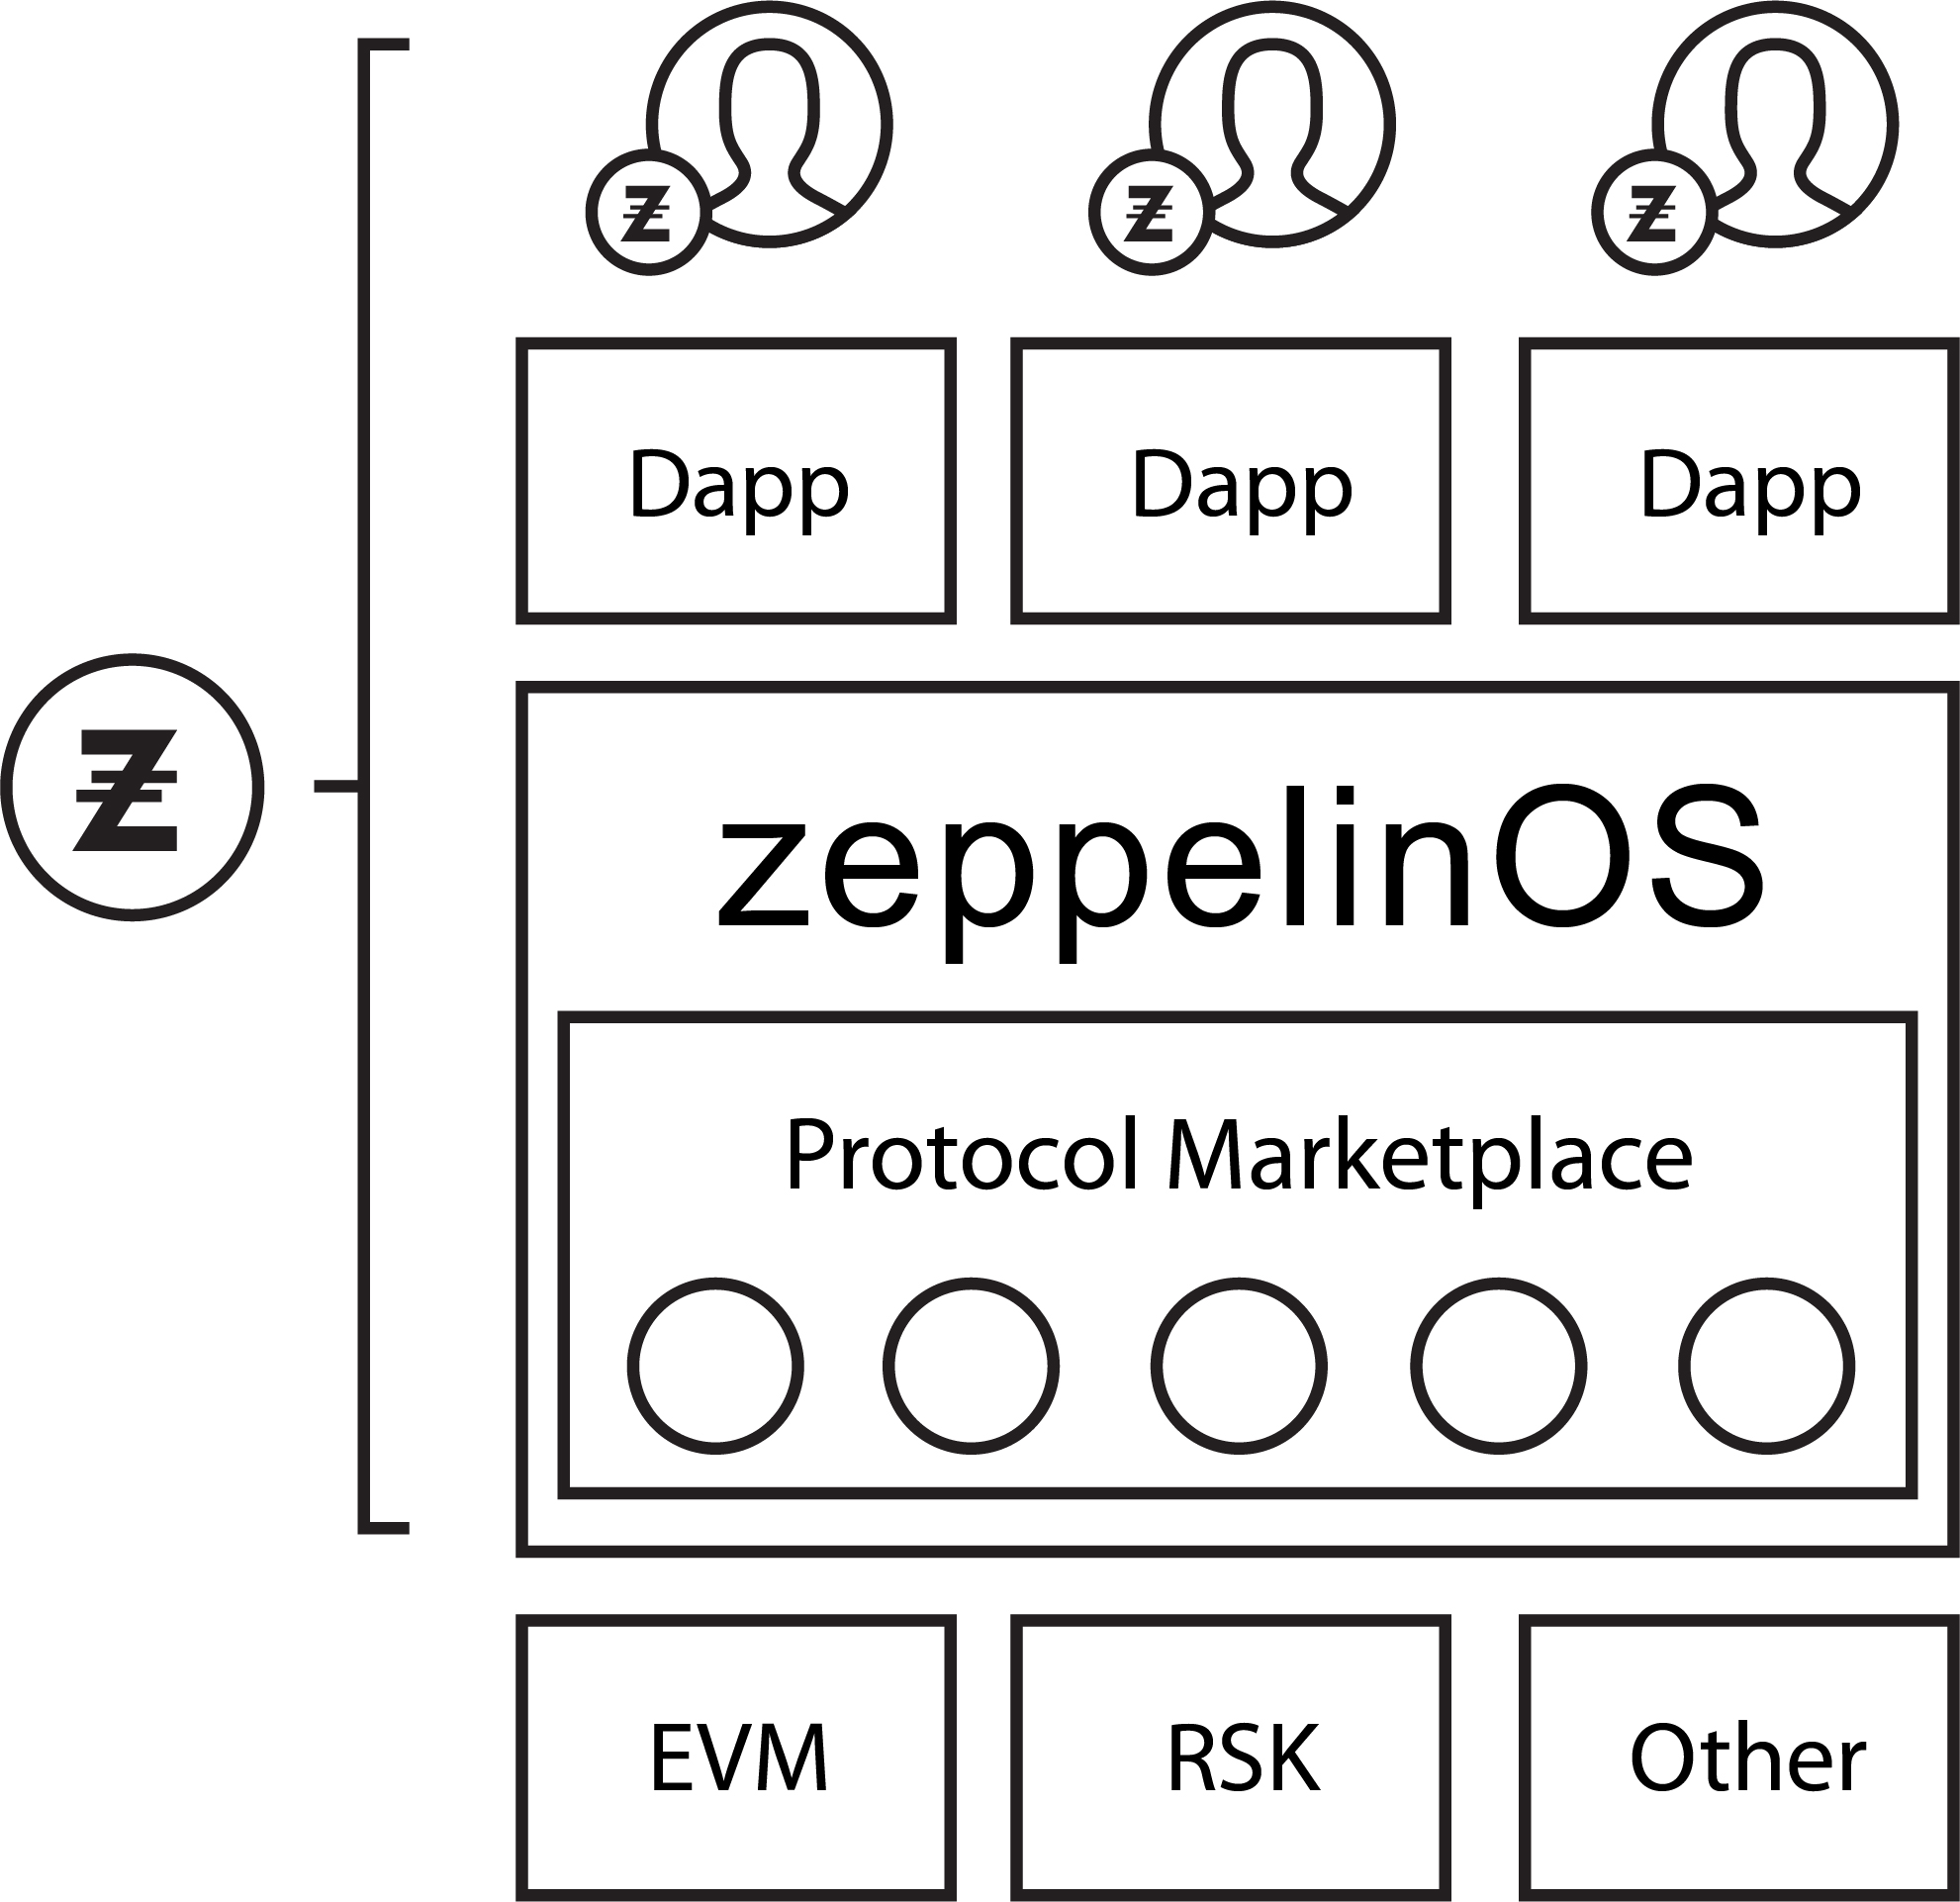
\includegraphics[width=0.4\linewidth]{images/image5.jpg}
  \caption{ZEP in relation to zeppelinOS stack.}
\end{figure}

\subsection{Utility}

\subsubsection{End-user}

Applications built on zeppelinOS will likely make use of various
external protocols to deliver services to users of said applications.
Usually this would require the user to hold tokens of each respective
protocol being used, making for a less than ideal user experience. The
ZEP token will significantly streamline the end-user experience, by
allowing users to perform all operations by using just ZEP tokens.
This end-user use-case will drive demand and increased
decentralisation, leading to a healthier, more robust network.

This isn't to say that applications built on zeppelinOS could not be
operated with other tokens as well, but settlements between tokens will
happen using the liquidity created with ZEP.

\subsubsection{Developers}

Developers will not have to spend ZEP tokens to develop
applications on zeppelinOS. Developers will need to own ZEP only
when conducting testing of deployed applications on the mainnet if they
have built token functionality into their application.

Developers will benefit greatly from ZEP tokens functioning as the
standard token due to significantly simplified economics of
applications, increased security due to standardisation and improved
end-user experiences. ZEP, together with the protocol marketplace,
create a plug and play experience for the developer when integrating
various protocol services into a decentralised application. Previously
if a developer has wanted to utilise more than one protocol's service,
they have needed to either require the user to hold the token of each
respective service to operate the dapp or provide exchange
functionality.

Developers also benefit from the compatibility of zeppelinOS with any
underlying blockchain running a virtual machine, essentially
future-proofing their applications. In addition, developers get easy
access to an existing ZEP-holding userbase and, in the future, end-user
facing distribution channels for applications built on zeppelinOS.

\begin{figure}
  \centering
  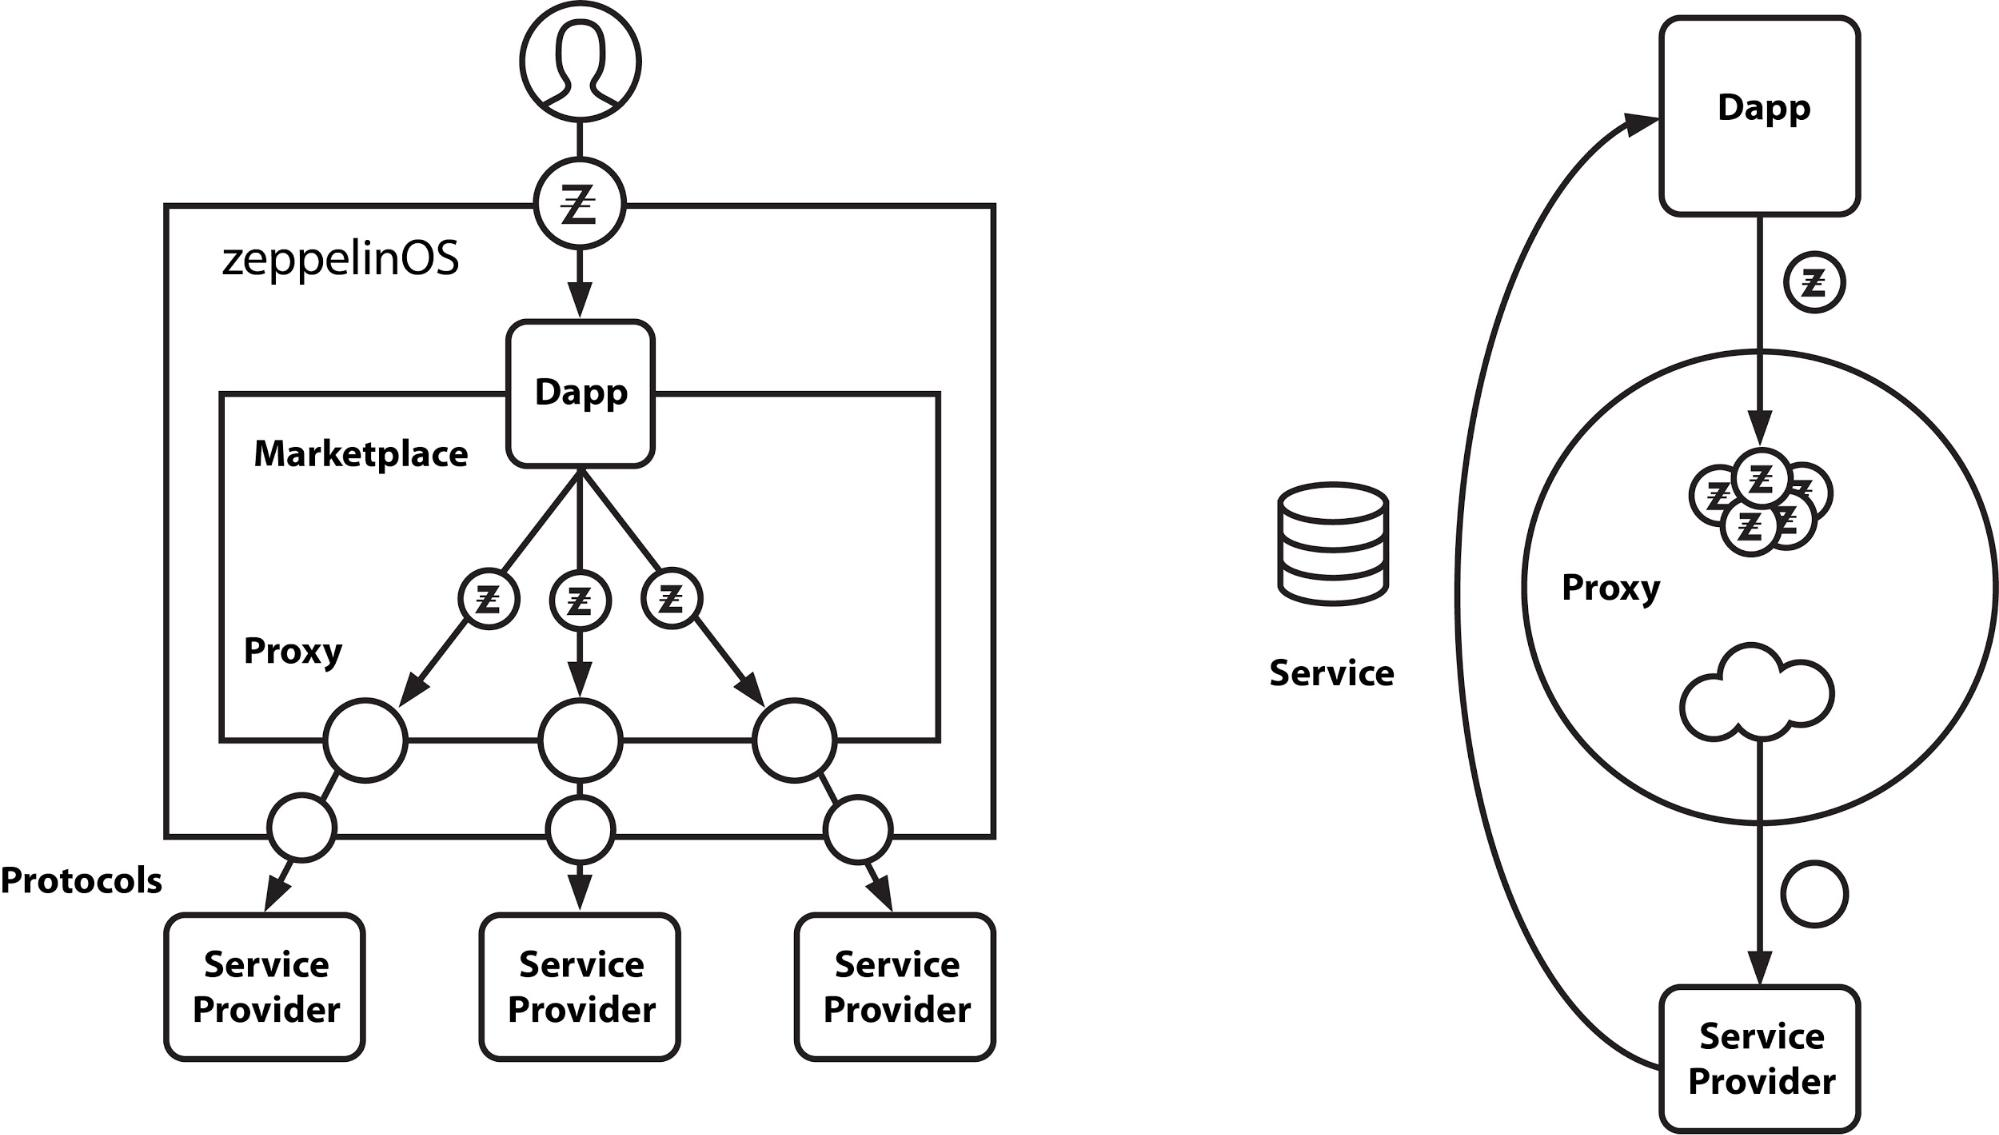
\includegraphics[width=0.75\linewidth]{images/image2.jpg}

  \caption{End-to-end token interactions.}
\end{figure}

\subsection{Governance}

In the context of zeppelinOS, governance mainly refers to the action of
upgrading or patching the Kernel code. This is achieved with a vouching
mechanism where network participants can stake (lock up) ZEP tokens to
vouch for a new version of the Kernel. Upgrading to a new version is
free, so this vouching mechanism is primarily a way for the network to
indicate the latest, qualified version of the Kernel and reward the
developers via a portion of staked ZEP going to said developers.

Conceptually, there are two distinct actions a Kernel user can
perform with regards to the upgrade mechanism:

\begin{enumerate}[label=\arabic*)]
  \item
    To change their contract's used kernel version from $V$ to $V'$. 
  \item
    To signal their approval or willingness to use $V'$ over $V$.
\end{enumerate}

Given 1) is very hard (or impossible) to tie into token mechanics
without forcing developers to hold ZEP tokens to use the Kernel,
we'll use 2) as a proxy of 1). To do so, we define the following
``vouch'' mechanic: ZEP token holders can signal their approval for a
specific Kernel version $V$ by lockingpart of their tokens and
specifying which version they vouch for. It's worth noting that the
Kernel is upgraded as a monolithic system and individual components
are not upgraded in a modular fashion, although this may be subject
to change in the future.

Locking tokens simply means the user cannot transfer or vouch other
versions with those same tokens. This doesn't mean tokens are locked for
a specific amount of time.

For example, given a Kernel with only versions v1.0.0 and v1.0.1, and 3
token holders with 100 ZEP tokens each, the following situation can
occur:

\begin{itemize}
  \item
    Holder A vouches for v1.0.0 with 50 ZEP tokens and v1.0.1 with 50 ZEP
    tokens.
  \item
    Holder B doesn't vouch for any version.
  \item
    Holder C vouches for v1.0.1 with 80 ZEP tokens.
\end{itemize}

In this example, if holders ABC make up a majority of vouching power in
the network, the new version 1.0.1 would be considered the latest
version accepted by the network, in the context of automatic
upgrades. It's important to note that users can manually change the
Kernel version their contracts use, making upgrades of the Kernel
opt-in. zeppelinOS will also provide tools for contracts to
automatically upgrade based on a policy set by the developer.

For the rest of the section, whenever we say ``use'' or ``upgrade'' in
relation to a version, we're referring to the vouching mechanic and not
actually using that version in their contracts.

\subsubsection{Mechanics}

The following mechanics govern the Kernel upgrade mechanism and
incentives.

Any developer can propose a new Kernel version upgrade, based on a
previously existing version. Creating this new version proposal has a
cost in ZEP tokens, as a way to prevent denial-of-service attacks
related to proposal submissions. Compensation to the
developer of a Kernel version is a function of the amount of tokens
vouching for that version. When a developer proposes a new version of
the Kernel, building upon a previous version, users can stop
vouching for the previous version in favor of the new one. Note:
Multiple versions of the Kernel can exist in parallel, creating a sort
of tree structure for versions.

Each of these vouch-change operations will compensate the new version's
developer according to a function of tokens vouched.

$\mathsf{change\_vouching}(v_1, v_2, t)$ will trigger a
$\mathsf{payout}(v_2, f(t))$, where $f$ is monotonically increasing over $t$,
the amount of tokens. Payouts may also include a time-lock or other additional
safety measures to ensure incentives are aligned.

Whenever a user vouches for a new version with t tokens, a fraction of
those tokens is sent to the developer as a reward. This causes
$\mathsf{change\_vouching}(v_1, v_2, t)$ to take $t$ tokens from $v_1$, give $f(t)$
to the developer, and lock $t - f(t)$ for $v_2$, where $f(t) = t * (1/k)$
where $k$ is a natural number. his definition of $f$ does not depend
on $\mathsf{total\_vouching\_tokens}$. This means the payout is a fraction of the
moved tokens, coming out of the voucher's balance.
Tokens given as reward to the developer have a time lock and are only
redeemable after a certain token amount threshold is met. During this lock-in
period, vouchers may decide to change their target version.

  Here's an example timeline of vouching changes:

\begin{longtable}[]{@{}llll@{}}
\toprule
\begin{minipage}[t]{0.22\columnwidth}\raggedright\strut
{Version}\strut
\end{minipage} & \begin{minipage}[t]{0.22\columnwidth}\raggedright\strut
{Vouch \% at $t_0$}\strut
\end{minipage} & \begin{minipage}[t]{0.22\columnwidth}\raggedright\strut
{Vouch \% at $t_1$}\strut
\end{minipage} & \begin{minipage}[t]{0.22\columnwidth}\raggedright\strut
{Vouch \% at $t_2$}\strut
\end{minipage}\tabularnewline \midrule
\begin{minipage}[t]{0.22\columnwidth}\raggedright\strut
{1.6.3}\strut
\end{minipage} & \begin{minipage}[t]{0.22\columnwidth}\raggedright\strut
{20}\strut
\end{minipage} & \begin{minipage}[t]{0.22\columnwidth}\raggedright\strut
{20}\strut
\end{minipage} & \begin{minipage}[t]{0.22\columnwidth}\raggedright\strut
{20}\strut
\end{minipage}\tabularnewline
\begin{minipage}[t]{0.22\columnwidth}\raggedright\strut
{2.0.1}\strut
\end{minipage} & \begin{minipage}[t]{0.22\columnwidth}\raggedright\strut
{80}\strut
\end{minipage} & \begin{minipage}[t]{0.22\columnwidth}\raggedright\strut
{70}\strut
\end{minipage} & \begin{minipage}[t]{0.22\columnwidth}\raggedright\strut
{0}\strut
\end{minipage}\tabularnewline
\begin{minipage}[t]{0.22\columnwidth}\raggedright\strut
{2.0.2}\strut
\end{minipage} & \begin{minipage}[t]{0.22\columnwidth}\raggedright\strut
{0}\strut
\end{minipage} & \begin{minipage}[t]{0.22\columnwidth}\raggedright\strut
{10}\strut
\end{minipage} & \begin{minipage}[t]{0.22\columnwidth}\raggedright\strut
{80}\strut
\end{minipage}\tabularnewline
\bottomrule
\end{longtable}

\begin{itemize}

  \item
    At time $t_0$ version 2.0.2 is released fixing a vulnerability in version
    2.0.1.

  \item
    At time $t_1$ a user with 10\% of the total vouching power moves their
    tokens from 2.0.1 to 2.0.2 ($\mathsf{change\_vouching}(2.0.1, 2.0.2, 10)$)
    which results in a compensation to the developers of 2.0.2
    ($\mathsf{payout}(2.0.2, f(10))$).

  \item
    At time $t_2$ the other user of 2.0.1 moves their tokens to 2.0.2, and this
    results in the compensation to the developers ($\mathsf{payout}(2.0.2, f(70))$).

\end{itemize}

\subsubsection{Contribution Dynamics}

We acknowledge that it's impossible to measure the value of a
contribution other than subjectively by the users of the OS. A change as
small as a single character can save millions of dollars, while a very
large changeset adding multiple contracts could be useless. There's no
objective way of measuring this from the code itself, only by how much
users adopt the changes.

As such, and as a result of the mechanics proposed above, each
proposed upgrade is rewarded equally, given the same amount of tokens
vouching for it. This will cause the developers proposing upgrades to
adapt each of their contributions to the expected reward, and the market
will determine whether the payout is fair by either vouching or not for
the contribution.

For instance, if the proposed upgrade is too small in terms of
value-added, the token holders will refrain from vouching for it, as the
payout to the developer would be unfair. This will cause developers to
avoid upgrade spamming, and incentivise them to band-up to submit bigger
contributions encompassing several small changes, with a payout address
set to a fund-splitting contract.

Also, note that any damage done by malicious actors in the system is
contained. Developers vouching for their own versions would end up
losing tokens, due to the associated costs of proposing new versions and
the tokens paid as part of the change\_vouching operation and malicious
users vouching for buggy versions, as an attempt to slow down
development or introduce vulnerabilities in the Kernel, will not be
followed by other users who will vouch for a different version in the
development tree.

All in all, since the motivation for vouching users is to maintain a
healthy development cycle of the OS and ensure the security of the
underlying Kernel libraries, we expect each vouching operation to be
done towards this end, regardless of the small number of tokens deducted
from the user's balance upon vouching.

\subsubsection{Development Bounties}

In order to guide the development of the zeppelinOS Kernel and
incentivize contributors to begin working on an issue, there will be a
platform for development bounties. In it, users can post their desired
features and place an upfront bounty for them, and do the same for bugs
that need to be fixed. The aim is for bounties to act as a pushing force
for the development of the Kernel, and a motivation for developers, in
addition to the usual reward that comes with the community vouching an
already released version. We aim to implement a delegated review process
for development bounty proposals, but initially this process will be
managed in a centralised manner.

As an end-to-end example of this process think of a developer that is
building a project on top of the zeppelinOS Kernel who runs into a need
for a type of smart contract that hasn't been built yet. Through the
platform, they will post a bounty of a given amount of ZEP tokens for
its development. Other developers might share the need for the feature,
and can add their own bounty on top. A developer will see this bounty
and announce that they began working on the feature. Once it's
finished, a network delegate will review the
submission. If
the feature implementation is acceptable, the bounty will be released to
the developer and the feature will be submitted for normal Kernel
upgrade vouching. A small cut will be rewarded to the reviewer.

\begin{figure}
  \centering
  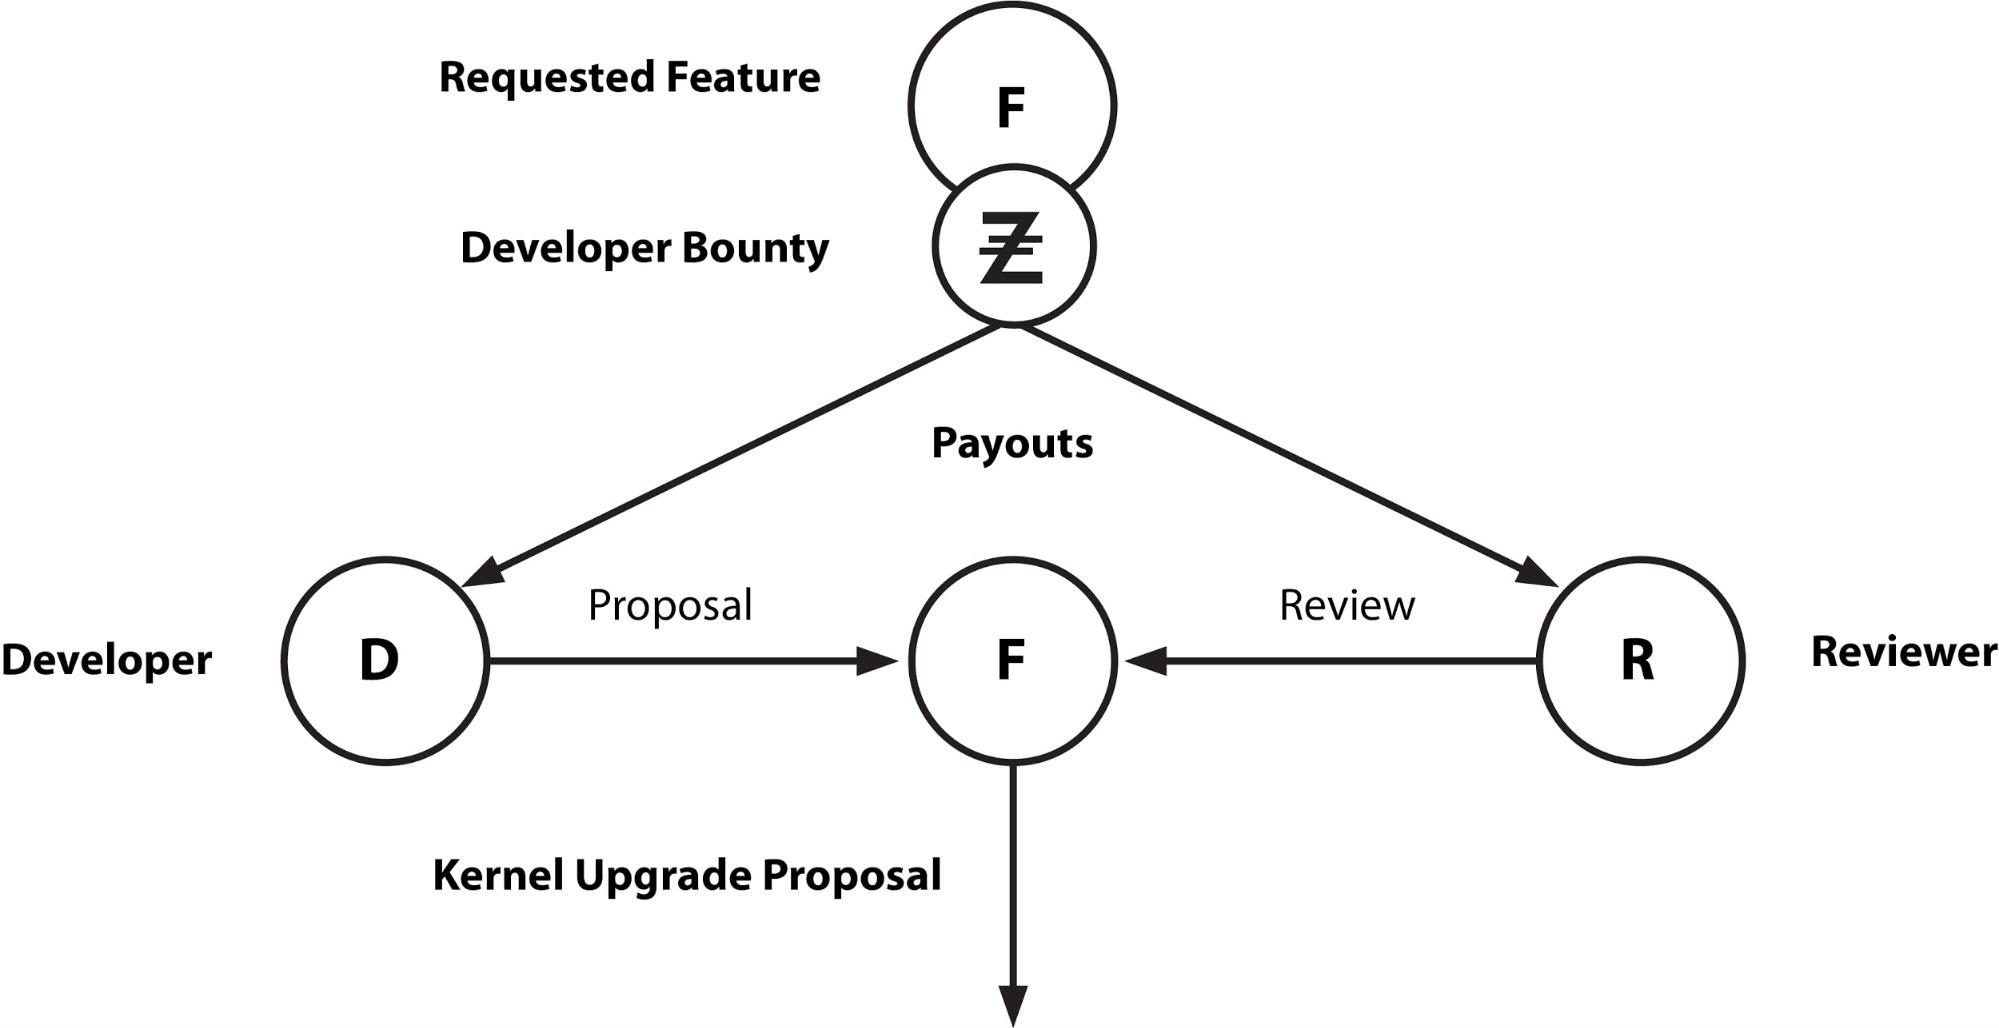
\includegraphics[width=0.75\linewidth]{images/image4.jpg}
  \caption{Developer bounty review and reward mechanism.}
\end{figure}

\paragraph{Considerations and Pending Challenges}

\begin{itemize}
  \item
    Specifics of voting process for choosing delegates are still
    undecided. Likely this will be similar to a delegated proof of stake
    system, where each token has a right to lock up tokens and thus give
    their vote for a specific delegate/reviewer.
  \item
    The incentives of the reviewer are easily misaligned with the network
    as the reviewer should be rewarded for every review, regardless of if
    the proposal is accepted or not. This creates an incentive for the
    reviewers to create large amounts of proposals that will be declined
    as the reviewer would still receive the reward, depleting the
    developer bounty
    pool.
\end{itemize}

\subsubsection{Automatic upgrade system}
\label{autoupgrade}

Users of the Kernel libraries will have the option to enable automatic
upgrades. For instance, users may specify that they use version \^{}1.2,
meaning the latest approved version among 1.2 and above, but below
2.0.

The latest approved version is defined based on the number of
tokens vouching for that version, with respect to its previous versions.
For example, given a Kernel version that specifies version \^{}1.2:

\begin{itemize}
  \item
    Kernel uses version 1.2, the latest one in the 1.x branch.
  \item
    Developers propose versions 1.3a and 1.3b as upgrades over 1.2.
  \item
    Over $X\%$ of vouching in the 1.x branch moves to 1.3a (where $X$ is to
    be defined), signalling that 1.3 is strongly backed by the community.
  \item
    The proxy to the Kernel 1.x branch is updated to point to version 1.3.
  \item
    Kernel automatically starts using features from 1.3.
\end{itemize}

These upgrades are optional for Kernel users, as they may choose to
switch manually to 1.3 after reviewing the new version themselves,
regardless of the vouching of that version.

\begin{figure}
  \centering
  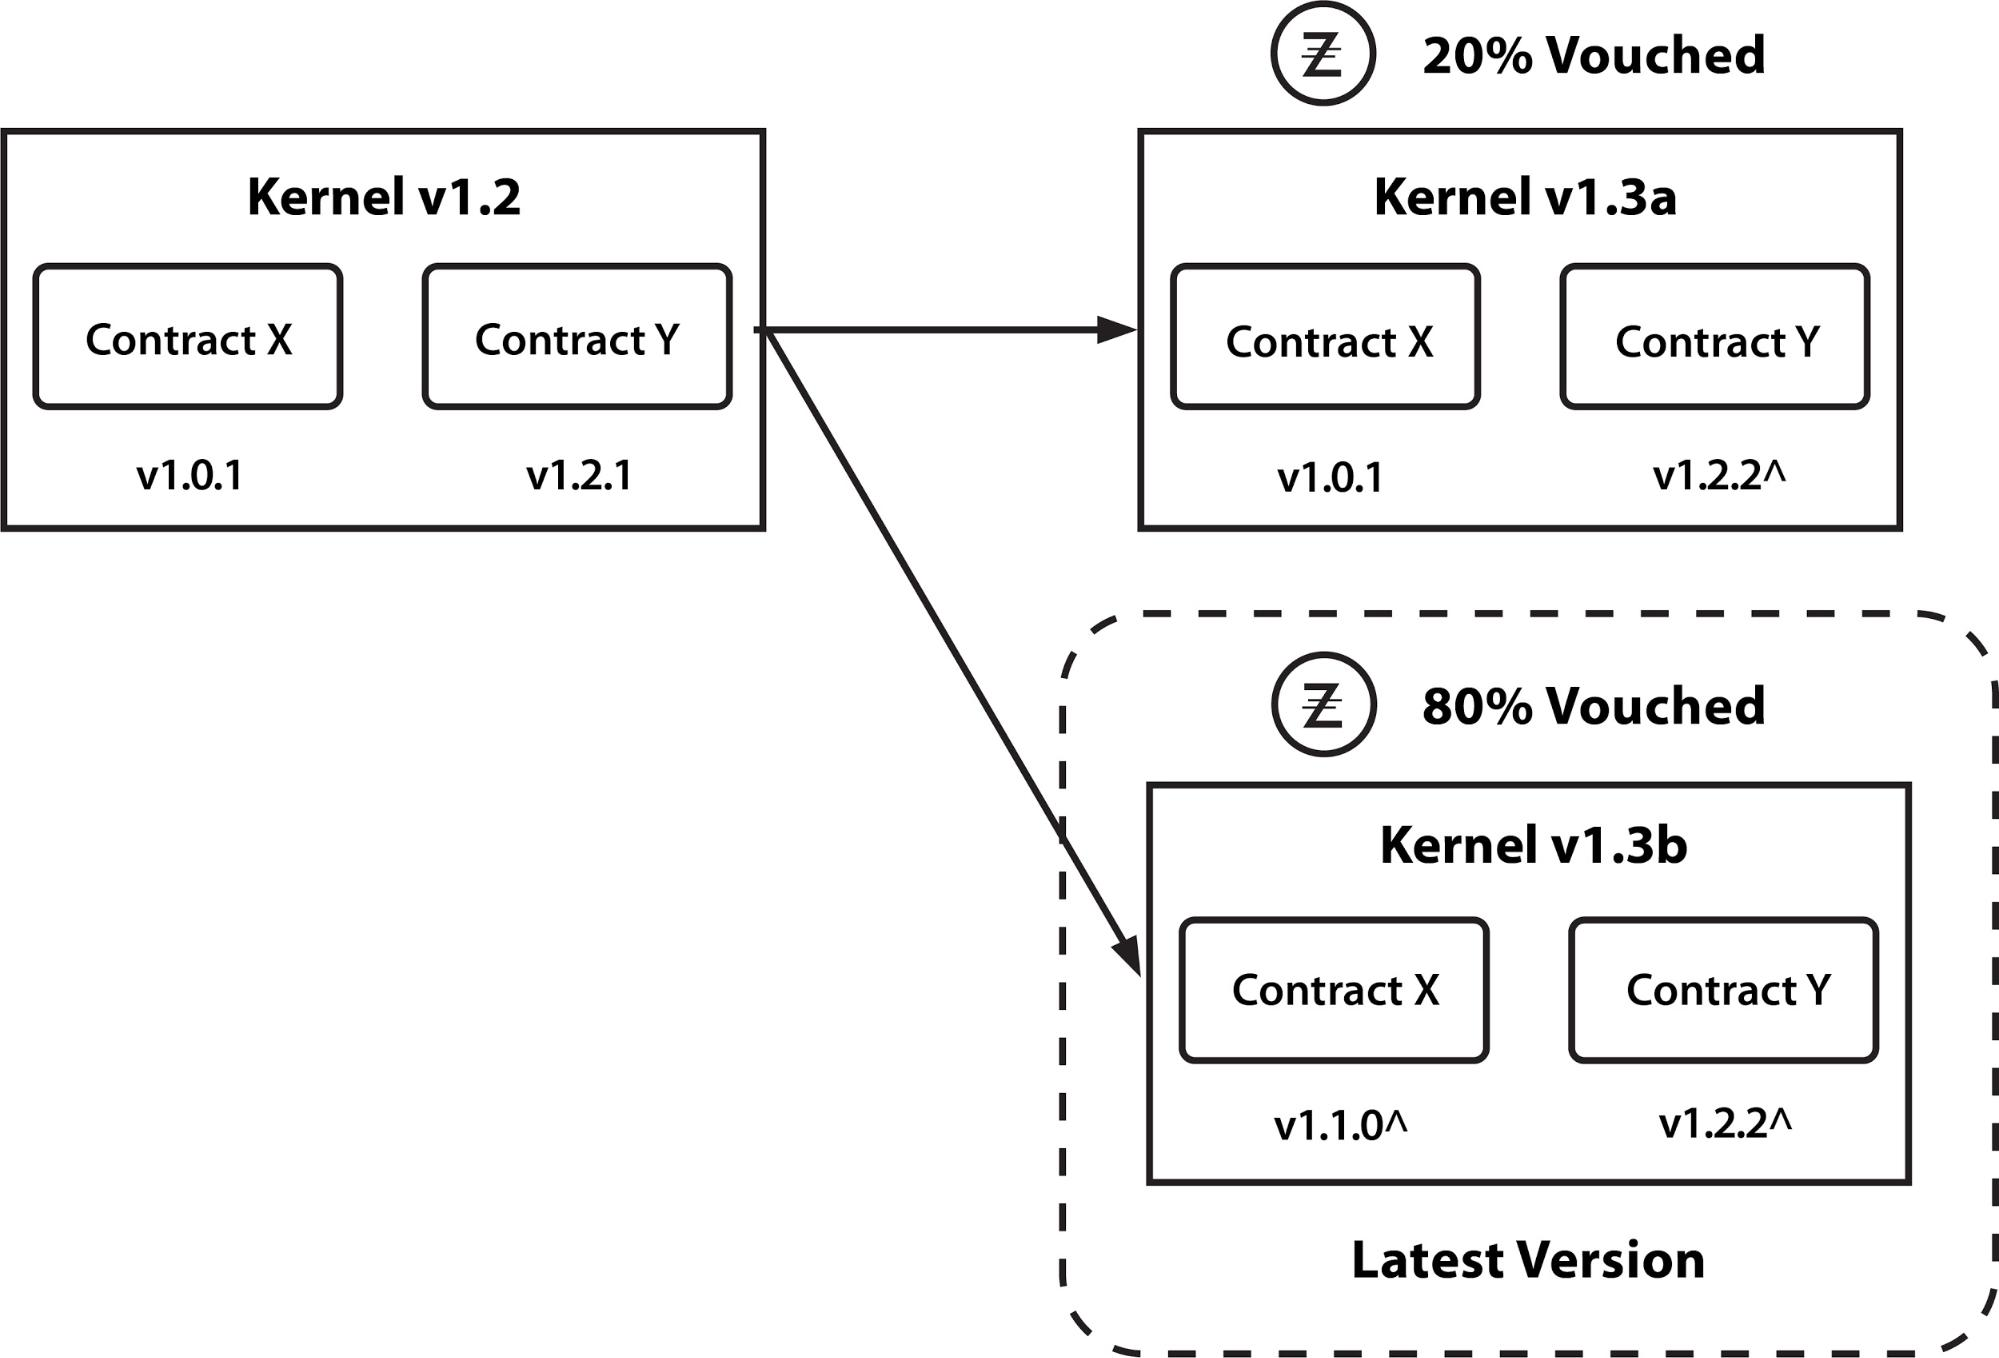
\includegraphics[width=0.75\linewidth]{images/image1.jpg}
  \caption{Illustration of automatic upgrade mechanism for example in section~\ref{autoupgrade}}
\end{figure}

\clearpage

\appendix

\section{Comprehensive list of token role in different
elements of the OS}

Summary of ZEP token usage by component or feature.

\begin{longtable}[]{@{}p{0.32\linewidth}p{0.32\linewidth}p{0.32\linewidth}@{}}
\toprule
\textbf{Section} & \textbf{Sub-Section} & \textbf{Actors and token
usage}\tabularnewline
\midrule
\endhead
\begin{minipage}[t]{0.32\columnwidth}\raggedright\strut
\textbf{zeppelinOS Kernel}\strut
\end{minipage} & \begin{minipage}[t]{0.32\columnwidth}\raggedright\strut
\textbf{Security Patches and Continuous Improvement}\strut
\end{minipage} & \begin{minipage}[t]{0.32\columnwidth}\raggedright\strut
\textbf{Developers:} receive ZEP tokens as a result of user `vouching'
for their versions.

\textbf{Users:} vouch versions, giving ZEP rewards to developers.\strut
\end{minipage}\tabularnewline\cmidrule{2-3}
& \textbf{Shared bug bounties} & Bounties will be issued in
ZEP.\tabularnewline\midrule
\multirow{2}{\linewidth}{\textbf{Smart Contract Development Tools}} & \textbf{Attack Management} &
\emph{No token required.}\tabularnewline\cmidrule{2-3}
& \textbf{Upgrade Management} & \emph{No token required.}\tabularnewline\cmidrule{2-3}
& \textbf{Thin Deployments} & \emph{No token required.}\tabularnewline\midrule
\begin{minipage}[t]{0.32\columnwidth}\raggedright\strut
\textbf{Smart Contract Interaction Tools}\strut
\end{minipage} & \begin{minipage}[t]{0.32\columnwidth}\raggedright\strut
\textbf{Scheduling}\strut
\end{minipage} & \begin{minipage}[t]{0.32\columnwidth}\raggedright\strut
\textbf{People in need of async execution}: issue

ZEP token bounties.

\textbf{Scheduling agent}: receives ZEP token for executing.\strut
\end{minipage}\tabularnewline\cmidrule{2-3}
\begin{minipage}[t]{0.32\columnwidth}\raggedright\strut
\strut
\end{minipage} & \begin{minipage}[t]{0.32\columnwidth}\raggedright\strut
\textbf{Marketplace}\strut
\end{minipage} & \begin{minipage}[t]{0.32\columnwidth}\raggedright\strut
\textbf{Consumers:} access services using ZEP tokens.

\textbf{Service providers:} provide services and receive ZEP
tokens.\strut
\end{minipage}\tabularnewline\cmidrule{2-3}
& \textbf{State Channel Support} & \emph{No token
required.}\tabularnewline\cmidrule{2-3}
& \textbf{Blockchain Information Provider} & \emph{No token
required.}\tabularnewline\midrule
\textbf{Off-Chain Tools} & \textbf{Analytics \& Monitoring} & Users can
pay in ZEP or any other token.\tabularnewline\cmidrule{2-3}
& \textbf{Platform as a Service} & Users can pay in ZEP or any other
token.\tabularnewline\cmidrule{2-3}
& \textbf{Continuous Integration for Contracts} & Users can pay in ZEP
or any other token.\tabularnewline\cmidrule{2-3}
& \textbf{Automated Code Analysis} & Users can pay in ZEP or any other
token.\tabularnewline\cmidrule{2-3}
& \textbf{Developer Tools} & Users can pay in ZEP or any other
token.\tabularnewline
\bottomrule
\end{longtable}

\clearpage

\begin{thebibliography}{20}

\bibitem{evm}
EVM. Ethereum virtual machine. \url{http://ethdocs.org/en/latest/introduction/what-is-ethereum.html\#ethereum-virtual-machine}

\bibitem{proxylibs}
Manuel Araoz, Jorge Izquierdo. Proxy Libraries in Solidity. \url{https://blog.zeppelin.solutions/proxy-libraries-in-solidity-79fbe4b970fd}

\bibitem{openzeppelin}
OpenZeppelin. \url{https://openzeppelin.org/}

\bibitem{schneier}
A plea for simplicity. \url{https://www.schneier.com/essays/archives/1999/11/a\_plea\_for\_simplicit.html}

\bibitem{statechan}
State channels. \url{http://www.jeffcoleman.ca/state-channels/}

\bibitem{zeppelinsols}
Zeppelin Solutions. \url{https://zeppelin.solutions/}

\bibitem{apple}
Time for Apple to face the music? \url{http://newsvote.bbc.co.uk/1/hi/technology/7002612.stm}

\bibitem{heroku}
Heroku. \url{https://heroku.com}

\bibitem{ifttt}
IFTTT. \url{https://ifttt.com/}

\bibitem{ethereum}
Ethereum. \url{https://ethereum.org}

\end{thebibliography}

\end{document}
